\begin{block}{Distribution Estimation}
\centering
        \heading{Goal: Obtain the Best Distribution of $\lambda$} 
        \begin{itemize}
            \itembox{\bf \large Bayesian Context:} Regular Bayes insufficient, Hierarchical model required.
            \itembox{\bf \large Data Consistent:} Use data to construct observed distribution. 
        \end{itemize}

\end{block}

% \vspace{-0.5cm}

\begin{block}{Example}
\centering
Consider an exponential decay problem with uncertain decay rate:
\begin{equation*}
       u(t) = u_0\exp(-\lambda t), \; u_0 = 0.5 ,\; t=2
   \end{equation*}
\vspace{-0.25cm}

\begin{tabular}{c|c}
\toprule
\multirow{2}{*}{\textbf{Regular Bayes}} & 
$\prior \sim U[0,1]\; , \quad  \likelihood\qGivelam\sim N\left(Q\lam,\sigma^2\right) $ \\
                                        & $\bayes$ \\ 
\midrule
\multirow{3}{*}{\textbf{Hierarchical Bayes}}   &
        $\prior\hyper \sim \chi^2_1\; , \quad \alpha,\beta\in\Omega :=[0,\infty)\times[0,\infty)$ \\
        & $\prior\lamGiveH s\sim \text{Beta}\hyper, \quad \likelihood\qGivelam \sim N\left(Q\lam,\sigma^2\right)$ \\
        & $\Hbayes$ \\
\midrule
\textbf{Data Consistent} &  $\dci$\\
\bottomrule
\end{tabular}
\vspace{1.cm}
\heading{Plots of Concepts and Results}
% \begin{figure}
%         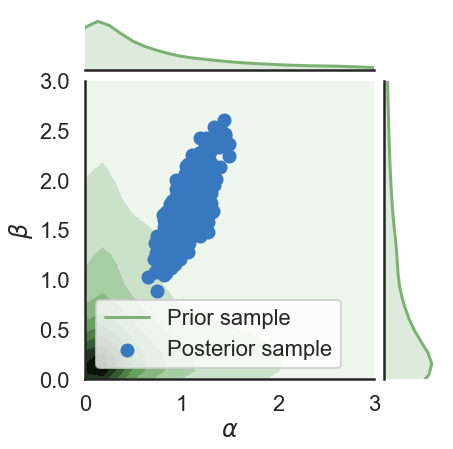
\includegraphics[width=10cm]{figures/distr_EX_hyper_param.png}
%         \vspace{-0.5cm}
%         \caption{$hyperspace$}
% \end{figure}
%\vspace{-1cm}
\begin{figure}
        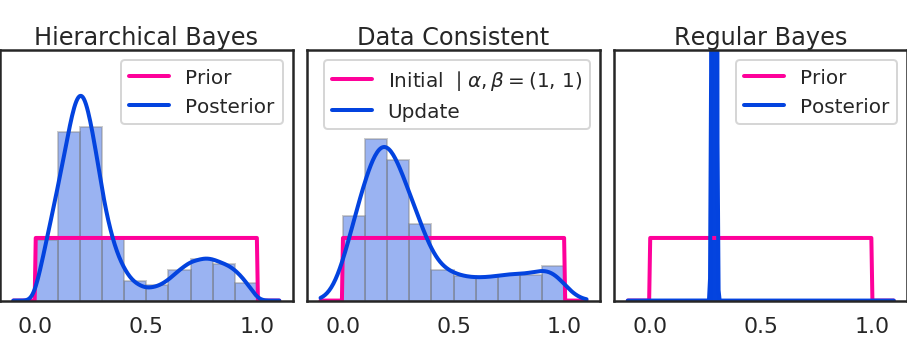
\includegraphics[width=32cm]{figures/distr_EX_lambda_space.png}
        \vspace{-0.5cm}
        \centering
        \caption{\large $\pspace$ Parameter Space }
\end{figure}

% \vspace{-0.5cm}

\begin{figure}
        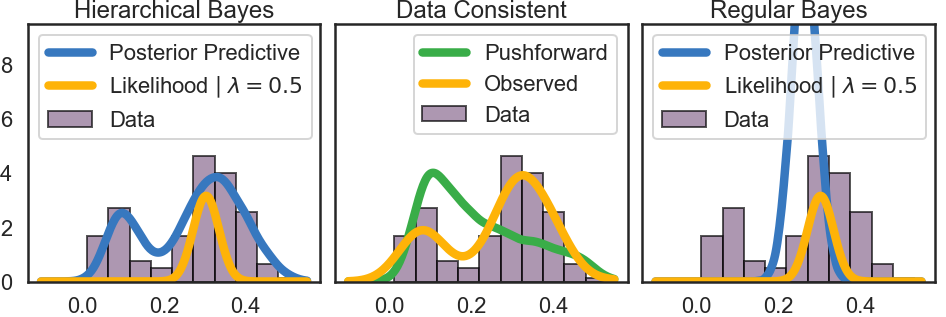
\includegraphics[width=32cm]{figures/distr_EX_data_space.png}
        \vspace{-0.5cm}
        \centering
        \caption{150 observations of data}
        \vspace{-0.5cm}
        \caption{\large $\dspace$ Data Space  }
\end{figure}


\end{block}

% \vspace{-0.5cm}

\begin{block}{Takeaways}

\centering
    \heading{Non-parametric method with less sampling}
%     \begin{equation*}
%             \dciP \quad \vline \quad \dci
%     \end{equation*}
    %\begin{equation*}
    %        \dci
    %\end{equation*}

\begin{figure}
        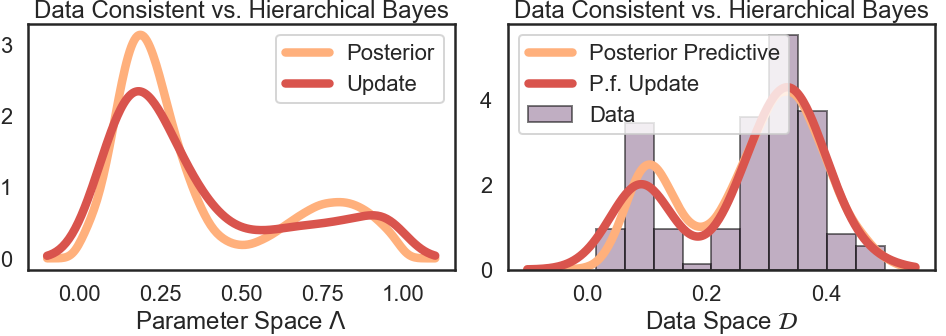
\includegraphics[width=30cm]{figures/distr_EX_comparison.png}
        \vspace{-0.5cm} 
        \caption{ }
    \end{figure}
\end{block}
%\textbf{Future research:} What are the connections to Dirchlet processes?
